%Engenharia de Software
%Relatório segundo sprint
\documentclass[12pt, a4paper, twocolumn]{article}

\usepackage[a4paper,top=2.5cm,bottom=2.554cm,left=2.554cm,right=2.554cm]{geometry}

\usepackage[portuguese]{babel}
\usepackage[utf8]{inputenc}
\usepackage{url}
\usepackage[pdftex]{graphicx}
\graphicspath{{./imagens/}}
\usepackage{color}
\usepackage{indentfirst}
\usepackage{mathtools}
\usepackage{caption}

\title{Relatório do Segundo Sprint\\ \textbf{Manipulação de tempo, Enviar e-mails e mensagens, Web Scraping e Manipulação de imagens}
		}
\author{Daniel Gomes, Érica Costa, Marcela Malaquias, Paulo Vicktor Felix}

\begin{document}

\maketitle

\begin{abstract}
Neste momento, focamos em aprender funções uteis para o desenvolvimento do nosso projeto final, portanto, os capítulos em questão serão de grande ajuda para que seja possível concluir o que desejamos.

Para o nosso objetivo, será necessário estabelecer uma comunicação entre o usuário e o Bot do telegram, logo, é útil que o bot tenha algumas funcionalidades diferenciadas, para se destacar entre os outros que já existem. Desse modo, iremos incluir em uma única plataforma funções como: verificar o clima, enviar um email, receber imagens de câmeras de segurança, acionar dispositivos remotos (Raspberry pi) e agendar tarefas.

\end{abstract}
\section{Manipulando o Tempo}
\subsection{O módulo time}
O relógio do sistema do computador está definido para uma data, hora e fuso horário específico. O módulo de time embutido permite que seus programas Python leiam o relógio do sistema para a hora atual. As time.time() e time.sleep()são as mais úteis no módulo de time.

\begin{itemize}
	\item Função time.time(): retorna o número de segundos desde aquele momento como um valor float.]
	\begin{figure}[htb!]
		\centering
		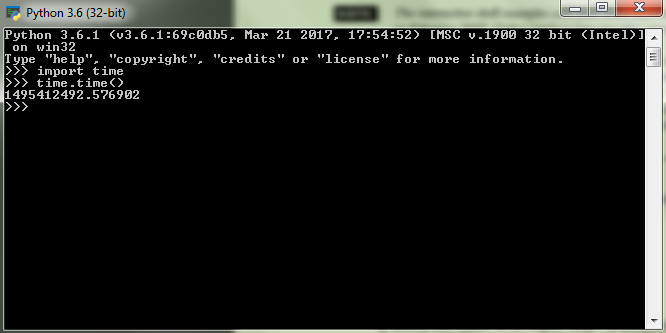
\includegraphics[scale = 0.45]{timetime.png}
		\caption{Função time.time}
	\end{figure}
	
	Obs: o valor de retorno é quantos segundos se passaram entre a época do Unix e o momento em que time.time() foi chamado.
	\item Função time.sleep(): para pausar o programa por um tempo, chame a função time.sleep()e passe o número de segundos que você deseja que o programa fique pausado. A função time.sleep() liberará seu programa para executar outro código - até que o número de segundos que você passou para time.sleep() tenha acabado. Por exemplo, se você inserir time.sleep(5) , verá que o próximo prompt não aparece até que cinco segundos tenham passado.
	\item Rounding numbers: Para tornar os valores float mais fáceis de trabalhar, pode-se encurtá-los com a função round(), que arredonda um float para a precisão especifica. Basta passar o número que se deseja arredondar, além de um segundo argumento opcional representando quantos dígitos após o ponto decimal que se deseja arredondá-lo. O segundo, round() arredonda seu número para o inteiro mais próximo.
	\begin{figure}[htb!]
		\centering
		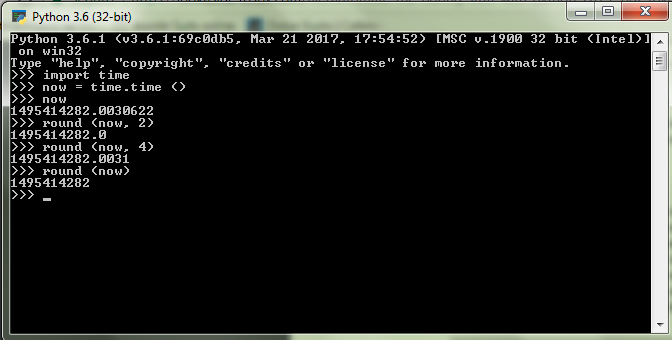
\includegraphics[scale = 0.45]{round.png}
		\caption{Uso de Rounding Numbers}
	\end{figure}
\end{itemize}
\subsection{O módulo datetime}
O módulo de time é útil para obter um timestamp de época Unix para trabalhar. Mas caso deseja exibir uma data em um formato mais conveniente, ou fazer aritmética com datas (por exemplo, descobrir qual data foi de 205 dias atrás ou data que é de 123 dias a partir de agora), pode-se deve usar o módulo datetime.
\begin{figure}[htb!]
	\centering
	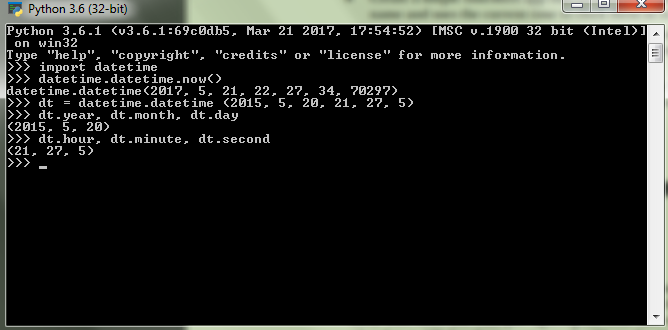
\includegraphics[scale = 0.45]{datetime.png}
	\caption{Resultado da aplicação de datetime }
\end{figure}
\section{E-mails e mensagens}
No capitulo 16 aprendemos a enviar e encontrar um email. Para enviar usamos funções como smtplib.SMTP para deternimar o tipo de uma conta de email e .login para logar em uma conta e tambem .semdmail para enviar texto. Ja para encontrar o email temos funções como .select\_folder para determinar onde iremos procurar o email (INBOX, lixo, enviados) temos tambem .search para buscar especificamente como a partir de uma data.
Segue exemplos de um programa enviando e outro procurando.
\begin{figure}[htb!]
	\centering
	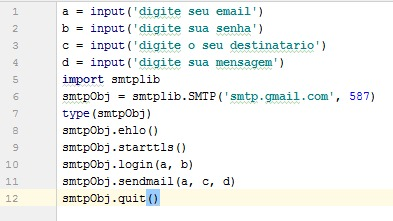
\includegraphics[scale = 0.5]{envia.jpeg}
	\caption{Resultado da aplicação de datetime }
\end{figure}
\begin{figure}[htb!]
	\centering
	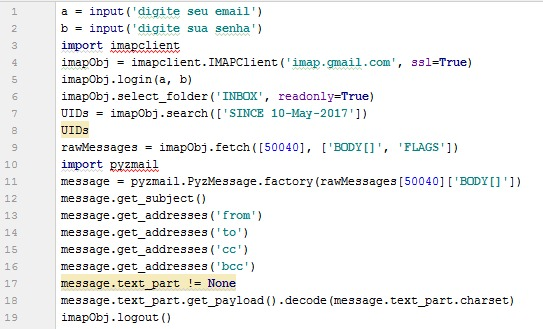
\includegraphics[scale = 0.38]{recebe.jpeg}
	\caption{Resultado da aplicação de datetime }
\end{figure}

\section{Web Scraping}
Utilizamos a Web Scraping para consultar o clima, por meio de uma API chamada OpenWeatherMap, que disponibiliza planos gratuitos e pagos para soluções em softwares. Assim, foi feito um cadastro no site da API e conseguimos uma licença gratuita para desenvolver a nossa aplicação com até 60 requisições por minuto.

\begin{figure}[htb!]
	\centering
	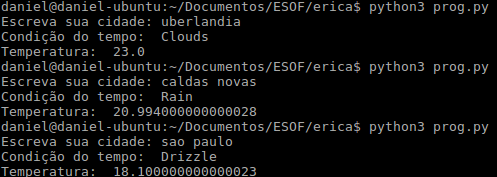
\includegraphics[scale = 0.45]{resultadoserica.png}
	\caption{Resultado da aplicação de WebScraping para Clima e Temperatura.}
\end{figure}

\section{Manipulando Imagens}
Para usar imagens em python, utilizaremos o módulo PIL. Este, conta com vasta aplicação, como cortar, rotacionar e salvar imagens. Abaixo, seguem exemplos de aplicação.
\begin{figure}[htb!]
	\centering
	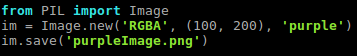
\includegraphics[scale = 0.55]{roxo.png}
	\caption{Criando uma imagem roxa.}
\end{figure}
\begin{figure}[htb!]
	\centering
	
\includegraphics[scale = 0.55]{purpleImage.png}
	\caption{Imagem criada nas dimensões escolhidas.}
\end{figure}

O próximo programa, abre uma imagem existente e muda o formato dela, no caso, estava em .jpg e mudou para .png.

\begin{figure}[htb!]
	\centering
	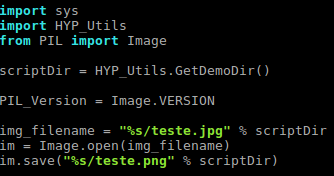
\includegraphics[scale = 0.60]{troca.png}
	\caption{Imagem criada nas dimensões escolhidas.}
\end{figure}




\section{Referências}
[1] SWEIGART, Al. "Automate the boring stuff with python", 2015. \\

[2] Documentation API OpenWeatherMap: \url{https://openweathermap.org/current}. Acesso em 20 de Maio de 2017, as 20h.

[3] Primeiros passos com PIL (IMB); \url{https://www.ibm.com/developerworks/community/blogs/fd26864d-cb41-49cf-b719-d89c6b072893/entry/primeiros_passos_com_pil_a_biblioteca_de_imagens_do_python2?lang=en}. Acesso em 15 de Maio de 2017, as 15h30.



\end{document}